\documentclass{article}
\usepackage[preprint]{neurips_2024}
\usepackage{amsmath,amssymb,booktabs,float,graphicx}
\usepackage[hidelinks]{hyperref}
\hypersetup{
  pdftitle={When Is a Smaller Model Enough? Training and Routing for CPU Sentiment Inference},
  pdfauthor={Anandteertha Rao},
  pdfsubject={ECE 592 / CSC 591 / ECE 492 course project report}
}
\makeatletter
\renewcommand{\@noticestring}{ECE 592 / CSC 591 / ECE 492 course project report, Fall 2026.}
\makeatother

\title{When Is a Smaller Model Enough?\\Training and Routing for CPU Sentiment Inference}
\author{Anandteertha Rao\\North Carolina State University}

\begin{document}
\maketitle

\begin{abstract}
I study how input shape, student training, and fallback policy affect batch-one CPU sentiment inference. Fixed-shape ONNX execution did not pass the break-even screen at any of 11 tested lengths. A four-layer distilled student with confidence-based fallback scored 90.48\% versus 91.06\% for the full teacher on 872 GLUE SST-2 sentences, and reduced paired median latency by 24.1\% within the memory budget. The original length-and-cost gate missed the one-point accuracy target. A tuned version got one more sentence right than confidence-only, used 12 fewer teacher calls, and reduced paired median latency by 2.02\% in a separate benchmark, while paired p95 increased by 3.14\%. On 720 previously unscored IMDb reviews, the tuned cutoff made 66 additional calls and lost four predictions relative to confidence-only. The results identify when extra routing information can help and how selection, cost estimates, and length distribution limit transfer. Code, protocols, and measurements are in the \href{https://github.com/anandteertha/length-aware-inference}{project repository}.
\end{abstract}

\section{Introduction}
On a CPU serving one sentence at a time, padding, model depth, and the cost of an extra model call can all affect latency. Fixing the input shape may help a runtime optimize a graph, but a graph sized for the next supported length may process more positions than a dynamic graph. Reducing the number of transformer layers removes work on every request, but can reduce accuracy. A cascade can recover some accuracy when its fallback rule identifies requests on which the teacher will help.

I study binary movie-review sentiment classification on GLUE SST-2 \citep{wang2018,socher2013}. The project targeted at most one percentage point of observed accuracy loss relative to the teacher, at least 15\% lower median end-to-end request time, and a peak resident-memory budget of 1,536 MiB. A fallback pays for a second inference and can replace a correct student prediction with a wrong one. Token length can affect runtime, while whether it predicts teacher benefit beyond the student's confidence is an empirical question.

This study makes three contributions.
\begin{itemize}
  \item I separated padding cost from shape specialization and tested when the latter paid for the former under two CPU backends.
  \item I compared truncation, supervised fine-tuning, and distillation, then measured a trained student-first cascade against the full teacher under explicit deployment budgets.
  \item I evaluated length, teacher cost, and routing cutoffs with matched-call replays, paired CPU timings, and an external audit, and examined cost-weighted training and INT8 as distinct ways to change the tradeoff.
\end{itemize}

\section{Related work}
Knowledge distillation transfers predictive information to smaller models \citep{hinton2015,sanh2019}. DeeBERT exits early inside one transformer \citep{xin2020}, while CascadeBERT uses calibrated decisions across complete models \citep{li2021}. \citet{jitkrittum2023} characterize optimal deferral in terms of the difference in expected correctness between models and describe conditions under which confidence-based deferral works or fails. Cascade-aware training changes how the smaller model learns its role in the combined system \citep{wang2024}. My contribution is a controlled empirical study of CPU shape, training, and routing tradeoffs for a particular teacher--student pair, using length-dependent measured cost as a routing input and end-to-end runtime as the evaluation outcome.

\section{Methods}
\subsection{Input shape and the teacher baseline}
The teacher is the public six-layer DistilBERT sentiment classifier fine-tuned on SST-2 \citep{sanh2019,checkpoint}. I pinned the checkpoint and tokenizer revision and used its dynamic FP32 ONNX export as the deployment baseline. Fixed variants use the same weights. The break-even screen used 24 previously unused SST-2 training examples at each of 11 exact lengths and three process blocks per backend and fixed capacity. I compared natural-length dynamic, bucket-padded dynamic, and equally padded fixed graphs in ONNX Runtime (ORT) and OpenVINO. This screen's p95 includes padding and inference and excludes tokenization, routing, and model loading. Within a block, padding cost equals padded-dynamic p95 minus natural-dynamic p95. Specialization gain equals padded-dynamic p95 minus fixed p95 at the same capacity. Net gain is specialization gain minus padding cost. The screen required positive net gain in every block and at least 5\% median paired p95 reduction, with numerical and resource checks passing.

\subsection{Student training}
The three- and four-layer students start with the teacher's embeddings, the first three or four transformer layers, and its classifier. The three-layer control keeps the copied weights unchanged. The supervised run updates weights using cross-entropy with the true label. For the distilled students I use
\begin{equation}
 \mathcal L = \tfrac12 \operatorname{CE}(y,p_s)
 + \tfrac12 T^2\,D_{\mathrm{KL}}\!\left(
     \operatorname{softmax}(z_t/T)\,\Vert\,\operatorname{softmax}(z_s/T)\right),
 \qquad T=2.
\end{equation}
Here \(z_s,z_t\) are the student and teacher logits and \(p_s=\operatorname{softmax}(z_s)\). Training used 8,192 examples, batch size 16, AdamW with learning rate \(2\times10^{-5}\), two epochs, and seed 2027. I chose checkpoints by accuracy on 1,024 separate development examples. A prespecified rule triggered the four-layer distilled run when the best three-layer development result trailed the teacher by more than three points. The observed gap was 4.69 points. I exported the students to dynamic FP32 ONNX and checked their outputs against PyTorch.

\subsection{Teacher benefit and routing}
\begin{figure}[H]
  \centering
  \setlength{\fboxsep}{6pt}
  \(\fbox{\textsf{Tokenize}}\ \longrightarrow\
    \fbox{\textsf{Run student}}\ \longrightarrow\
    \fbox{\textsf{Score and compare with cutoff}}\)
  \par\smallskip
  \(\text{Score below cutoff}\ \longrightarrow\ \text{Return student}
  \qquad
    \text{Score at or above cutoff}\ \longrightarrow\ \text{Run and return teacher}\)
  \caption{Student-first execution. A fallback incurs teacher inference in addition to the student work already done.}
  \label{fig:flow}
\end{figure}
The student runs on every request (Figure~\ref{fig:flow}). On 2,048 labeled fitting examples I set \(g_i=\mathbf{1}[\hat y_{t,i}=y_i]-\mathbf{1}[\hat y_{s,i}=y_i]\). This gives \(+1\) for a teacher fix, \(-1\) for harm, and zero when correctness is unchanged. I fit ridge regression with penalty 10 on non-intercept coefficients using the student logit margin \(m=|z_{s,1}-z_{s,0}|\), log length \(\ell=\log_2 L\), and their interaction.

With standardized features \(\tilde m,\tilde\ell\), the gate calls the teacher when \(S_\alpha(x)\geq\tau\).
\begin{equation}
 S_\alpha(x) = \frac{\widehat G(x)}{C(L)^\alpha} =
 \frac{\beta_0+\beta_1\tilde m+\beta_2\tilde\ell+\beta_3\tilde m\tilde\ell}{C(L)^\alpha}.
 \label{eq:score}
\end{equation}
Here \(C(L)\) is the median teacher-only ONNX inference time on gate-fit rows, represented numerically in milliseconds. The costs were 9.61, 17.91, and 27.83 ms for 3--16, 17--32, and 33+ tokens. The original rule used \(\alpha=1\). At \(\alpha=0\), the score uses estimated gain alone. The confidence-only control uses a one-feature ridge score with a negative coefficient on margin, equivalent to keeping the teacher fallback when the margin is at or below its cutoff. Neither policy needs teacher output to make the decision.

On 1,024 distinct calibration examples I evaluated score thresholds corresponding to fallback targets of \(0, 0.1, 0.2, 0.3, 0.4, 0.5, 0.7,\) and \(1\). For each original rule, I selected the smallest estimated mean extra teacher cost among candidates within one accuracy point of the teacher. Extra cost was zero when the student answer was kept. The fit and calibration partitions were disjoint from student training, student development, each other, and the 872-row GLUE validation split. They came from the SST-2 training split used to fine-tune the released teacher. I froze both original policies before validation. Later routing studies explicitly repurposed the GLUE validation labels for development.

\subsection{Exponent and cutoff search}
I first reduced the cost exponent while keeping the learned gain model fixed. I then checked score crossings between requests from different cost bins to identify which equal-call rankings could change with the exponent. Equal-call replays use the top requests in the full cohort and are an offline diagnostic. To select usable per-request cutoffs, I also tested a grid of 51 exponents from 0 to 1 and 91 calibration fallback targets from 2.5\% to 25\%. Each target is converted to a score quantile on the original calibration set. The realized call rate depends on the workload.

On GLUE, I required at least 786 of 872 correct (within one point of the teacher), at most 161 calls, and estimated added mean teacher cost at most 3.66 ms per request, the confidence-only value. I ranked eligible settings by accuracy, estimated cost, and call count, in that order. I froze the GLUE-selected policy for replay on 1,812 Stanford SST binary test sentences after excluding neutral examples and normalized matches to GLUE train or validation. I also identified a retrospective choice using both splits. I froze both policies before scoring 720 previously unscored IMDb test reviews, balanced by label and three token-length groups and filtered against earlier IMDb samples \citep{maas2011}.

\subsection{Resident timing and follow-up experiments}
Each fresh CPU process loaded both ONNX sessions, used four ORT intra-op threads per session with spinning disabled, and warmed both sessions on 32 requests. The original comparison timed all 872 natural-length requests at batch size one on an Intel Core i5-1334U laptop. In a separate AC-powered benchmark, the two-split grid choice and confidence-only ran the same 872 requests in four paired blocks, alternating which policy ran first. Request order matched within each pair. End-to-end latency includes tokenization, routing when applicable, and inference. I summarize latency within each process and compare the matched processes within blocks. Model startup is separate and memory is measured while both sessions are resident. The descriptive paired accuracy bootstrap uses 10,000 resamples of aligned examples.

The cost-weighted training extension applied weights of 0.537, 1.000, and 1.554 to the distillation term in the three length bins and retained the four-layer training settings. Its external comparison used 1,000 balanced IMDb test reviews of at most 512 tokens without truncation. The exploratory INT8 extension applied ORT dynamic QInt8 weight quantization to the four-layer student's MatMul and Gemm operations with per-channel quantization and reduced range disabled \citep{ortquant}. It first kept the FP32 cutoff, then fitted INT8-specific cutoffs on the archived Stanford set before replay on GLUE and the reused 1,000-review IMDb cohort.

\section{Results}
\subsection{Fixed shapes and training ablations}
None of the 11 tested lengths passed the fixed-shape screen in either backend. For example, at 33 tokens in one OpenVINO block, padding to 64 added 18.71 ms to p95 and specialization recovered 6.48 ms, leaving a net loss of 12.23 ms. The result applies to the tested lengths and settings. The archived break-even map reports the three-block range at each length.

\begin{table}[H]
\centering
\caption{Training ablation on the same 872 SST-2 validation examples.}
\label{tab:student}
\begin{tabular}{lrr}
\toprule Model & Correct & Accuracy (\%)\\
\midrule
Three-layer truncation & 645 & 73.97\\
Three-layer supervised & 735 & 84.29\\
Three-layer distilled & 739 & 84.75\\
Four-layer distilled & 765 & 87.73\\
Six-layer teacher & 794 & 91.06\\
\bottomrule
\end{tabular}
\end{table}
Supervised training recovered 90 correct predictions over truncation (Table~\ref{tab:student}). Distillation added four more correct predictions at three layers in this run. The four-layer distilled student recovered 26 more than its three-layer distilled counterpart. The study uses one seed and does not include a four-layer supervised control. The four-layer student still fell 3.33 points short of the teacher.

\subsection{Frozen cascade comparison}
\begin{table}[H]
\centering
\caption{Resident CPU comparison. Median and p95 are medians of their process-level summaries in milliseconds. Paired gain is the median of three within-block reductions in median latency versus teacher-only.}
\label{tab:cascade}
\begin{tabular}{lrrrrr}
\toprule Policy & Correct & Teacher calls & Median & p95 & Paired gain\\
\midrule
Teacher only & 794 & 872 & 27.92 & 78.22 & ---\\
Student only & 765 & 0 & 18.32 & 41.84 & 33.9\%\\
Length and cost & 779 & 121 & 20.45 & 54.61 & 23.2\%\\
Confidence only & 789 & 161 & 21.20 & 67.29 & 24.1\%\\
\bottomrule
\end{tabular}
\end{table}
The confidence-only control met the observed criteria with a 0.57-point accuracy loss, latency reductions of 10.1\%, 24.1\%, and 30.3\% across the paired blocks, and peak working set of about 928 MiB (Table~\ref{tab:cascade}). Its accuracy difference versus the teacher has a descriptive paired 95\% interval of \([-1.61,+0.46]\) percentage points, which crosses the one-point loss limit. Confidence cascade p95 was lower in two blocks and higher in one.

The original length-and-cost gate corrected 24 student mistakes and introduced 10 errors, for 14 net corrections. It missed the accuracy target by losing 1.72 points relative to the teacher. Its matched-call and length-stratified diagnostics are reported below.

\subsection{Where full cost penalization lost accuracy}
Table~\ref{tab:length} shows why fewer calls alone were insufficient. At 33 or more tokens, the teacher got 186/208 correct versus 174/208 for the student. Calling the teacher on all 208 would fix 18 errors and introduce six. Confidence-only recovered nine of the twelve net corrections with 45 calls. The original cost-aware gate sent just 13 of these cases and recovered five net corrections. For requests with positive estimated gain, dividing by a larger cost suppresses their score even when the teacher often helps in that group.

\begin{table}[H]
\centering
\caption{Full-model correctness and routed teacher calls by token length on the 872 GLUE SST-2 sentences. The student is the four-layer distilled FP32 model. Original and tuned use cost exponents 1 and 0.16 respectively.}
\label{tab:length}
\setlength{\tabcolsep}{5pt}
\begin{tabular}{rrrrrrr}
\toprule
 & & \multicolumn{2}{c}{Correct if used alone} & \multicolumn{3}{c}{Teacher calls}\\
\cmidrule(lr){3-4}\cmidrule(l){5-7}
Tokens & Cases & Student & Teacher & Original & Confidence & Tuned\\
\midrule
3--16 & 197 & 185 & 183 & 33 & 17 & 11\\
17--32 & 467 & 406 & 425 & 75 & 99 & 88\\
33+ & 208 & 174 & 186 & 13 & 45 & 50\\
\bottomrule
\end{tabular}
\end{table}

Softening the cost exponent to 0.75 raised the original frozen policy from 779 to 786 correct and increased calls on the longest group from 13 to 35. Its total calls rose from 121 to 161. At a common offline budget of 161, the original, softened, and confidence rankings got 782, 786, and 789 correct, respectively. The fixed softened rule met the one-point accuracy budget, and five paired CPU runs showed mixed timing results. The wider continuous exponent sweep found no stable interval that improved on confidence-only at equal calls on both short-text splits.

\subsection{Grid search, latency, and transfer}
Of 4,641 fixed-cutoff policies, 186 met the GLUE accuracy, call, and estimated cost conditions. Only seven beat confidence-only accuracy, all by one example (Figure~\ref{fig:grid}). The GLUE choice used exponent 0.10 and cutoff 0.09240. It used 20 fewer calls on GLUE, then lost three correct predictions on Stanford while making 45 fewer calls. The two-split choice used exponent 0.16 and cutoff 0.07545. It preserved the Stanford count with 28 fewer calls (Table~\ref{tab:transfer}). Stanford's labels helped select the 0.16 policy, so the tie is retrospective.

\begin{figure}[H]
  \centering
  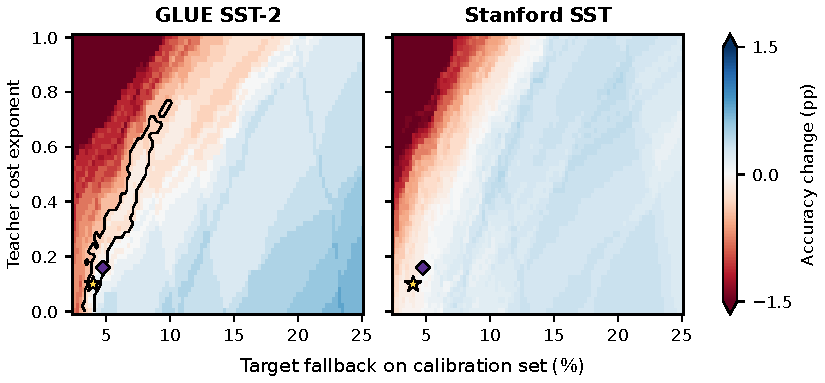
\includegraphics[width=\linewidth]{report/figures/gate-grid.pdf}
  \caption{Accuracy change in percentage points (pp) relative to confidence-only on two short-text splits. Blue indicates gains and red indicates losses. Black contours outline the eligible GLUE grid cells. The star marks the GLUE-only choice and the diamond marks the two-split choice. A target sets a fixed calibration score cutoff, so realized call rates vary by split.}
  \label{fig:grid}
\end{figure}

\begin{table}[H]
\centering
\caption{Correct predictions and teacher calls for the same fixed cutoffs on GLUE, Stanford, and previously unscored IMDb reviews. Each cell gives correct predictions followed by calls.}
\label{tab:transfer}
\begin{tabular}{lrrr}
\toprule
Policy & GLUE (872) & Stanford (1,812) & IMDb (720)\\
\midrule
Confidence-only & 789 / 161 & 1,670 / 337 & 647 / 147\\
GLUE choice, \(\alpha=0.10\) & 790 / 141 & 1,667 / 292 & 643 / 213\\
Two-split choice, \(\alpha=0.16\) & 790 / 149 & 1,670 / 309 & 643 / 213\\
\bottomrule
\end{tabular}
\end{table}

In the separate four-block timing run, the 0.16 gate made 12 fewer calls on the same workload and got one more prediction right. The median of process medians was 10.46 ms for the tuned gate and 10.53 ms for confidence-only. The corresponding p95 summaries were 29.46 and 28.67 ms. Within-block median latency fell in three pairs and rose in one, for a median paired change of \(-2.02\%\). The p95 rose in three pairs, for a median paired change of \(+3.14\%\) (Figure~\ref{fig:paired}). These relative changes summarize the paired blocks and therefore differ from ratios of the two aggregate latencies. Peak working sets were 928.0 and 927.7 MiB, respectively. Every timed prediction and route matched the replay. The tuned gate routed five more 33+ token requests and 17 fewer shorter requests than confidence-only. Timing aggregates do not identify whether this shift caused the higher p95.

\begin{figure}[H]
  \centering
  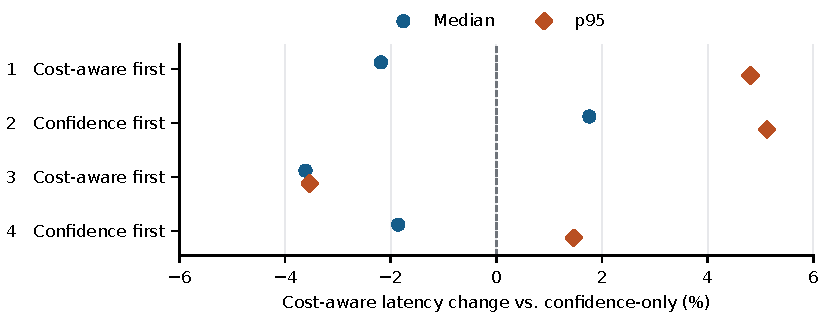
\includegraphics[width=\linewidth]{report/figures/paired-latency.pdf}
  \caption{Within-block latency changes for the frozen 0.16 policy relative to confidence-only. Each row compares the two policies on the same 872 requests in separate processes. Values left of zero favor the 0.16 gate. Markers show process-level estimates and first-policy order, with no request-level confidence intervals.}
  \label{fig:paired}
\end{figure}

On the 720-review IMDb audit, the two tuned policies made identical decisions. They included every confidence-only fallback plus 66 more. The extra calls fixed three student mistakes and introduced seven new ones. The net loss was four correct predictions (\(-0.56\) points, descriptive paired 95\% interval \([-1.39,+0.28]\) points). In this sample 718 reviews fell into the single 33+ token cost bin, where changing the exponent only rescales the predicted-gain scores. The fixed cutoff and gain model therefore determined the transfer outcome within almost the entire sample. IMDb and Stanford were accuracy and routing evaluations, without measured request latency for these policies.

\subsection{Alternative routing signals}
I screened additional formulas that shrank the length and interaction terms, applied additive cost, or used predicted class. The best GLUE formula only gained one correct prediction over confidence-only at 161 calls, then lost one at equal calls on the separate Stanford set. On a separate 720-review IMDb sample, two frozen scores using margin and length each gained one correct prediction at 174 calls by avoiding the same teacher-induced error. On another 960-review sample, a fix-minus-harm score matched confidence-only at 222 calls. Its fixed cutoff scored 867/960 with 206 calls versus 865/960 with 222 for the original confidence cutoff. At an offline confidence budget of 206 calls, the advantage narrowed to one correct prediction. These point results show where a policy can improve by avoiding teacher errors and also how much of an apparent gain depends on the operating point.


\subsection{Cost-weighted training and INT8 follow-up}
The cost-weighted student scored 832/1,000 on IMDb versus 843/1,000 for uniform distillation. The paired difference was \(-1.1\) points, with a descriptive 95\% interval of \([-2.6,+0.4]\). On reused SST-2 validation it gained five correct predictions overall and lost three in the longest stratum it was designed to help. Its end-to-end CPU latency was not measured.

The planned direct quantization of the archived four-layer ONNX graph failed during ONNX shape inference with a 768-versus-2 dimension conflict. The prespecified attempt ended at conversion. In a separately labeled exploratory repair, I cleared the intermediate tensor annotations before quantization. This left the FP32 operators, weights, and input and output definitions intact. The original and stripped FP32 graphs agreed within \(10^{-4}\) absolute and relative tolerance on probe inputs of 3, 16, 32, 55, 211, and 512 tokens. The repaired input allowed ORT to construct the INT8 candidate with the original quantizer settings.

The student graph shrank from 211.6 MB to 124.8 MB, a 41.0\% reduction in serialized bytes. On SST-2 the INT8 student scored 760/872 (87.16\%), versus 765/872 (87.73\%) for FP32. Its frozen confidence cascade scored 785/872 (90.02\%), versus 789/872 (90.48\%) for FP32 and 794/872 (91.06\%) for the full teacher. The exact loss against the teacher was \(100(794-785)/872=1.032\) points, exceeding the one-point target. Quantization changed 27 student predictions and 61 routing decisions, raising teacher calls from 161 to 206. A smaller serialized graph alone cannot establish lower request latency or process memory.

On the reused IMDb sample, each student got 843/1,000 correct, with 40 predictions differing between FP32 and INT8. The planned resident timing run requires AC power and remains pending. The accuracy audit already rules out this INT8 cascade at the tested cutoff under the project's observed acceptance criteria.


\section{Discussion}
\subsection{When alternative policies should help}
\paragraph{Length and teacher specialization.}
Student confidence measures the student's uncertainty. The relevant quantity for routing is the teacher's chance of fixing an error minus its chance of replacing a correct answer with an error, conditional on what the gate can see. Length can improve this estimate if reviews of different lengths show different teacher benefit \emph{at comparable student margins}. A teacher trained for a particular genre, longer context, or a specific error type could make that difference large enough to matter. The present long-text average supports checking for such a signal. It cannot distinguish length from differences in difficulty or composition. In a separate diagnostic, the least-confident fifth of Stanford had teacher net gains of 1.54, 15.14, and 13.27 percentage points at up to 16, 17--32, and 33--64 tokens respectively. The middle bin led the longest of these bins even within this broad confidence group. Across the same diagnostic cohorts, the least-confident fifth gained about 11--12 points overall, while the remaining four fifths gained at most 0.35 points. That concentration explains why the margin was a strong baseline. To improve on it, new features must distinguish fixes from harms among requests that are comparably uncertain, especially near the cutoff.

\paragraph{Average cost and tail latency.}
For an additive mean-cost objective, suppose \(G(x)=\mathbb{E}[g\mid x]\) is expected net correctness gain, \(C(x)\) is expected incremental teacher time, and \(\lambda\) is the cost of one millisecond in correctness units. A fallback improves the objective when \(G(x)-\lambda C(x)>0\). Confidence remains competitive when this net value is already ordered by margin. Cost-aware routing can add value when teacher time varies substantially at similar margins, and when measured costs reflect the deployment workload. The power-law score in Equation~\ref{eq:score} is a heuristic for exploring this tradeoff. Summing per-bin medians estimates added work. It cannot determine p95, which depends on where slow requests land in the full latency distribution. A tail-sensitive deployment should measure latency by length and fallback outcome under representative load and select the policy under an explicit p95 constraint. Cutoffs should be calibrated on the target domain, especially when most of its requests collapse into one cost bin.

\paragraph{Input shape and student optimization.}
Fixed shapes are promising when requests cluster near a supported capacity and the measured specialization gain exceeds padding and routing overhead. Stable warm sessions and an affordable memory footprint are prerequisites for that comparison. The tested buckets offer no such demonstrated route. INT8 showed that a faster graph can still change the ranking of uncertain cases. Replacing FP32 would require an INT8-specific gate that meets the accuracy target on unseen labels, followed by matched timing. Cost-weighted training could help when the expensive group contains enough learnable student errors to justify shifting training emphasis. A cascade-aware training objective could instead prioritize the cases the student will actually keep. Neither quantization-aware training nor joint training of the student and gate was evaluated here.

\subsection{Limitations and scope of claims}
\textbf{Data and selection.} Gate fitting and calibration used SST-2 training examples from the public teacher's fine-tuning split. The partitions were separate from one another and from the student's training data. The teacher's training exposure can still distort estimates of its example-level benefit. The original operating points were frozen before row-level GLUE evaluation. Later sweeps used GLUE as development data, and Stanford was reused across the project and used to choose the 0.16 policy. A one-example gain after a large grid search does not establish superiority. The fresh IMDb audit excluded previously scored reviews, but it is label- and length-balanced and capped at 160 tokens. It does not represent all IMDb traffic, and differences between datasets cannot be attributed to length alone. A stronger replication would keep gate fitting and calibration out of teacher training, predeclare the policy and comparisons, and use a separate test set sampled for the target workload.

\textbf{Systems and training.} The CPU results use one laptop, batch-one requests, warm sessions, and a few paired process blocks. Repeated requests within a process are not independent hardware replications. I did not measure throughput under load, energy, or GPU performance. Training used one seed and had no four-layer supervised control, leaving the separate effects of depth and distillation unresolved at that size. I did not time the recalibrated INT8 gate, cost-weighted checkpoint, or external grid replays end to end.

\textbf{Claim boundary.} The accuracy budget is an observed engineering criterion. The original paired interval includes a loss larger than one point, so the study cannot establish population noninferiority. It also does not establish a universal length boundary, superiority over other models or tasks, or a novel cascade principle. Its contribution is the measured interaction between padding, model capacity, routing accuracy, and latency in this setting.

\section{Conclusion}
Selective fallback let the four-layer student meet the project's observed accuracy, latency, and memory goals on SST-2. The tuned cost-aware gate found a narrower advantage on that workload, exchanging a small median improvement and fewer calls for slower tail responses, with weaker transfer to longer IMDb reviews. Confidence-only is the better-supported default for these models. A targeted gate is most plausible when the deployment workload contains a reproducible source of teacher benefit beyond student margin, and when the saved computation is verified against the latency metric that the deployment actually cares about.


\section{Code and reproduction}
The \href{https://github.com/anandteertha/length-aware-inference#readme}{README} gives setup and the full command order. With the dynamic teacher prepared, train and export the students and fit the original gate.
\begin{verbatim}
uv run --locked python scripts/train_students.py
uv run --locked python scripts/train_capacity.py
uv run --locked python scripts/fit_gate.py
uv run --locked python scripts/export_students.py
\end{verbatim}
With the verified FP32 exports, run the grid, the IMDb audit, and the timing comparison. The final command redraws the report figures.
\begin{verbatim}
uv run --locked python scripts/plot_gate_grid.py
uv run --locked python scripts/plot_gate_grid.py --imdb
uv run --locked python scripts/time_gate_grid.py
uv run --locked python tools/plot_report_routing.py
\end{verbatim}
The \href{https://github.com/anandteertha/length-aware-inference/tree/main/results/student-study/gate-grid}{grid and transfer archive} and \href{https://github.com/anandteertha/length-aware-inference/tree/main/results/student-study/gate-grid-timing}{paired timing archive} include frozen plans, logits, and per-process results.

\clearpage
\begin{thebibliography}{10}
\bibitem[Hinton et~al.(2015)]{hinton2015}
G. Hinton, O. Vinyals, and J. Dean. Distilling the knowledge in a neural network.
\href{https://arxiv.org/abs/1503.02531}{arXiv:1503.02531}, 2015.
\bibitem[Hugging Face(n.d.)]{checkpoint}
Hugging Face. DistilBERT base uncased finetuned SST-2.
\href{https://huggingface.co/distilbert/distilbert-base-uncased-finetuned-sst-2-english/tree/714eb0fa89d2f80546fda750413ed43d93601a13}{Model card and pinned checkpoint}.
\bibitem[Jitkrittum et~al.(2023)]{jitkrittum2023}
W. Jitkrittum, N. Gupta, A. K. Menon, H. Narasimhan, A. S. Rawat, and S. Kumar.
When does confidence-based cascade deferral suffice?
\href{https://papers.neurips.cc/paper_files/paper/2023/hash/1f09e1ee5035a4c3fe38a5681cae5815-Abstract-Conference.html}{NeurIPS}, 2023.
\bibitem[Li et~al.(2021)]{li2021}
L. Li, Y. Lin, D. Chen, S. Ren, P. Li, J. Zhou, and X. Sun. CascadeBERT: Accelerating inference of pre-trained language models via calibrated complete models cascade.
\href{https://aclanthology.org/2021.findings-emnlp.43/}{Findings of EMNLP}, 2021.
\bibitem[Maas et~al.(2011)]{maas2011}
A. L. Maas, R. E. Daly, P. T. Pham, D. Huang, A. Y. Ng, and C. Potts.
Learning word vectors for sentiment analysis.
\href{https://aclanthology.org/P11-1015/}{ACL}, 2011.
\bibitem[ONNX Runtime(n.d.)]{ortquant}
ONNX Runtime. \href{https://onnxruntime.ai/docs/performance/model-optimizations/quantization.html}{Quantize ONNX models}. Documentation.
\bibitem[Sanh et~al.(2019)]{sanh2019}
V. Sanh, L. Debut, J. Chaumond, and T. Wolf. DistilBERT, a distilled version of BERT: smaller, faster, cheaper and lighter.
\href{https://arxiv.org/abs/1910.01108}{arXiv:1910.01108}, 2019.
\bibitem[Socher et~al.(2013)]{socher2013}
R. Socher, A. Perelygin, J. Wu, J. Chuang, C. D. Manning, A. Ng, and C. Potts.
Recursive deep models for semantic compositionality over a sentiment treebank.
\href{https://aclanthology.org/D13-1170/}{EMNLP}, 2013.
\bibitem[Wang et~al.(2018)]{wang2018}
A. Wang, A. Singh, J. Michael, F. Hill, O. Levy, and S. R. Bowman.
GLUE: A multi-task benchmark and analysis platform for natural language understanding.
\href{https://aclanthology.org/W18-5446/}{BlackboxNLP}, 2018.
\bibitem[Wang et~al.(2024)]{wang2024}
C. Wang, S. Augenstein, K. Rush, W. Jitkrittum, H. Narasimhan, A. S. Rawat, A. K. Menon, and A. Go.
Cascade-aware training of language models. \href{https://arxiv.org/abs/2406.00060}{arXiv:2406.00060}, 2024.
\bibitem[Xin et~al.(2020)]{xin2020}
J. Xin, R. Tang, J. Lee, Y. Yu, and J. Lin.
DeeBERT: Dynamic early exiting for accelerating BERT inference.
\href{https://aclanthology.org/2020.acl-main.204/}{ACL}, 2020.
\end{thebibliography}
\end{document}
